% Popout, alpha = 3
\begin{figure}
  \centering
    \makebox[\textwidth]{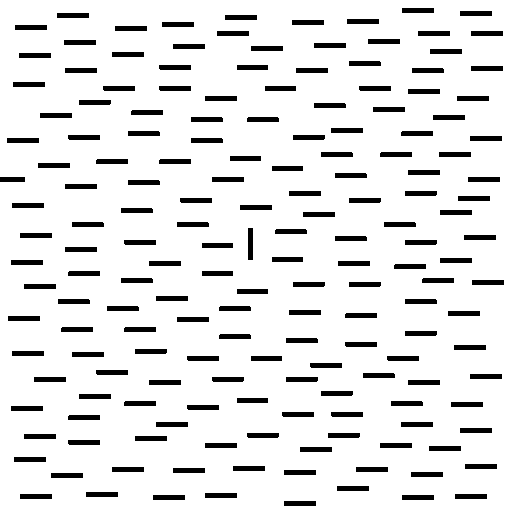
\includegraphics{./canny/popout}} \\
  \caption{Original popout image}
  \label{fig:popout}
\end{figure}

\begin{figure}
  \centering
    \makebox[\textwidth]{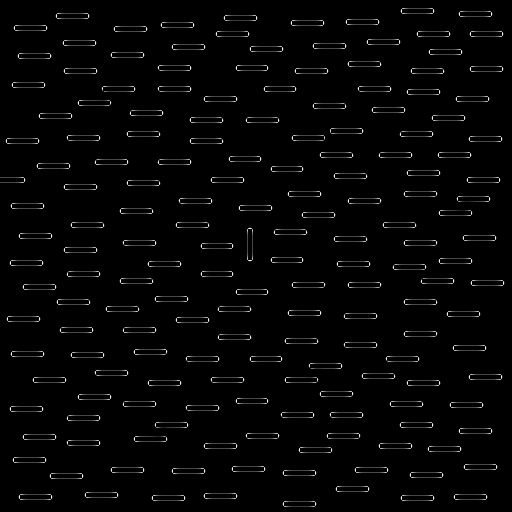
\includegraphics{./canny/popout_LINF_a3_k11_k24}} \\
  \caption{popout, Isotropic L-infinity norm. $\alpha$ = 3, K1 = 1, K2 = 4}
  \label{fig:popout_LINF_a3_k11_k24}
\end{figure}

\begin{figure}
  \centering
    \makebox[\textwidth]{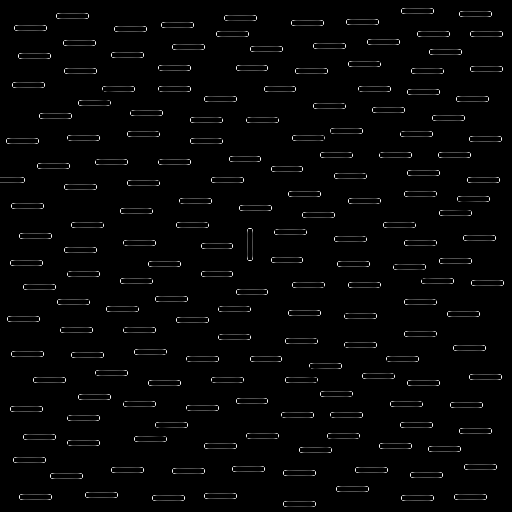
\includegraphics{./canny/popout_L1_a3_k11_k24}} \\
  \caption{popout, Isotropic L1 norm. $\alpha$ = 3, K1 = 1, K2 = 4}
  \label{fig:popout_L1_a3_k11_k24}
\end{figure}

\begin{figure}
  \centering
    \makebox[\textwidth]{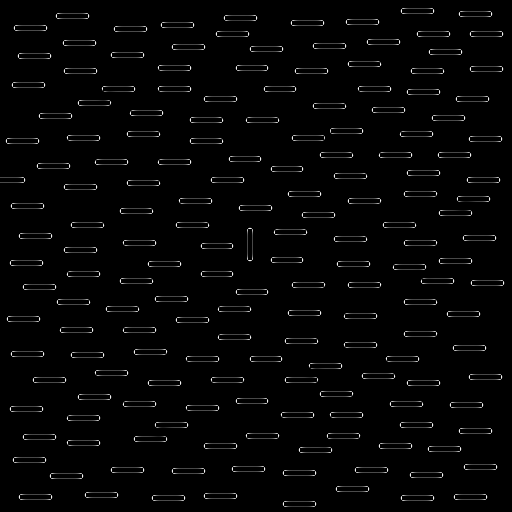
\includegraphics{./canny/popout_L2_a3_k11_k24}} \\
  \caption{popout, Isotropic L2 norm. $\alpha$ = 3, K1 = 1, K2 = 4}
  \label{fig:popout_L2_a3_k11_k24}
\end{figure}

\begin{figure}
  \centering
    \makebox[\textwidth]{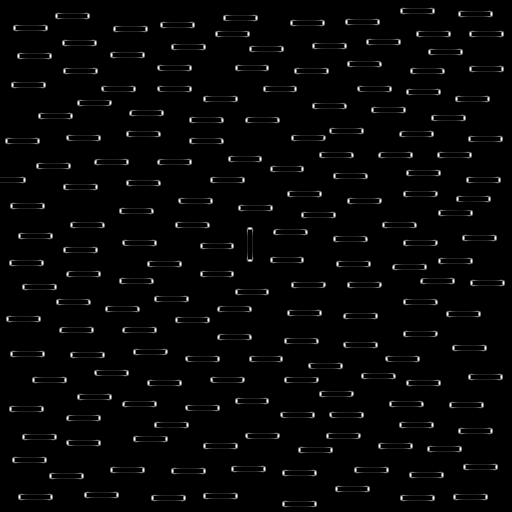
\includegraphics{./canny/popout_ANISO_a3_k11_k24}} \\
  \caption{popout, Anisotropic. $\alpha$ = 3, K1 = 1, K2 = 4}
  \label{fig:popout_ANISO_a3_k11_k24}
\end{figure}